\documentclass{bioinfo}
\usepackage{datetime}
\usepackage{float}
\usepackage{listings}
\usepackage{color}

\definecolor{mygreen}{rgb}{0,0.6,0}
\definecolor{mygray}{rgb}{0.5,0.5,0.5}
\definecolor{mymauve}{rgb}{0.58,0,0.82}


\lstset{ %
  backgroundcolor=\color{white},   % choose the background color
  basicstyle=\footnotesize,        % size of fonts used for the code
  breaklines=true,                 % automatic line breaking only at whitespace
  captionpos=b,                    % sets the caption-position to bottom
  commentstyle=\color{mygreen},    % comment style
  escapeinside={\%*}{*)},          % if you want to add LaTeX within your code
  keywordstyle=\color{blue},       % keyword style
  stringstyle=\color{mymauve},     % string literal style
}


\copyrightyear{2017} \pubyear{2017}

\access{Bioinformatics Report \\
Date: \today}
\appnotes{Graduate Assignment}

\begin{document} 
\firstpage{1}

\subtitle{Bioinformatics}

\title[Bio-informatics Assignment]{Protein Classification By feature extraction}
\author[Bio-informatics Assignment]{Sofiane MAHIOU}
\address{Computer Science, UCL, London, WC1E 6BT, UK}

\corresp{}

\history{}

\editor{}

\abstract{\textbf{Motivation :} The goal of this assignment is to provide an automated system that is able to classify proteins (Amino Acid sequences) into four classes each being a subcellular locations : \textbf{[Cytosolic, Secreted, Nuclear, Mitochondrial]}. The subcellular location is an important information as it provides more knowledge about the protein function, it is therefore, very helpful to be able to automatically extract that information for any given protein.\\
\textbf{Results :} Using a \textit{Random Forest Classifer} we manage to reach a \textbf{67\% cross-validation accuracy}.\\
\textbf{Improvements:} In order to improve the results of the classifier, deepening the feature extraction method seems to be the way to go. Another method would be to use neural network techniques.\\
\textbf{Contact:} \href{ucabsm1@ucl.ac.uk}{ucabsm1@ucl.ac.uk}\\
}

\maketitle

\section{Introduction}

Currently, There is a growing need for fully automated methods to analyse amino acid sequences. One of the process that need to be automated is \textbf{the identification of the protein's subcellular location}. This problem can be splitted into two sub problems :\\
\begin{itemize}
	\item \textbf{feature extraction: } the goal of this task is to choose the features that would allow an efficient classification, to be more precise, the chosen features should allow to easily seperate the sequences into classes or groups which will then be matched with the various subcellular locations 
	\item \textbf{classification: } once the features obtained, it is then necessary to choose a fitting classification algorithm that will use the various features selected as a \textit{vector representation} of each sequence that will then be fed to the classification algorithm during both training and testing.
\end{itemize}

It is however, possible to avoid splitting the problem into two sub-problems by using methods that have been designed to classify sequences of variables lengths such as :\\
\begin{itemize}
	\item \textbf{HMM} 
	\item \textbf{Recurrent neural networks \& Seq2Seq Models}
	\item \textbf{1D Convolutional Neural Networks}
\end{itemize}

Although these methods usually yield better results than the methods presented before, the results obtained are far harder to interpret as these systems behave as \textbf{"black boxes"} and it's quite difficult to identify what was \textit{learned}. \\

Therefore, the first approach was used in order to ease the analysis of the results and the task was splitted into a \textbf{feature-extraction} task and \textbf{classification} task. In order to identify what features might be useful to this problem, a research phase was realized where several research papers on the same subject have been studied, and used as a reference to select several features. 

% \enlargethispage{12pt}
\section{Sequence preprocessing : }
It seems important to mention that before proceeding the \textbf{feature extraction} phase, it was necessary to preprocess the data due to the presence of unexpected characters : \textbf{U, B, X} in the amino acid sequences. 

\begin{itemize}
	\item \textbf{X: } Given that "X" refers to "any amino acid" we randomly replace it by a given amino acid among the 20 amino acids
	\item \textbf{B: } "B" refers to either \textit{asparagine} and \textit{aspartic acid}. It is therefore automatically replaced by one or the other
	\item \textbf{U: } the "U" amino acid is simply removed from the sequence for lack of a better solution

\end{itemize}
 
 This preprocessing step, will only affect 64 sequences out of more than 9000, therefore these changes are unlikely to heavily influence the results but will allow and easier implementation of the various features.

\section{Feature Extraction}

We identify three different types of features:
\begin{itemize}
 	\item \textbf{Amino acids composition: } This refers to count or frequency of each amino acid in the sequence to analyse. 
	\item \textbf{Protein's properties: } This refers to the various chimical and biological properties that a given protein can have such as \textit{aromaticity, hydrophobicity, iso-electric point ...etc}
	\item \textbf{Subsequence-based features : } This refers to various existing methods that aim to extract relevant discriminative subsequences which \textit{presence or count} will then be used as features to classify the proteins
\end{itemize}

The goal will then be combine several features from each type in order to optimize the results of the classification. The process through which the features to extract were selected was mainly based on what several research papers on this field advised and recommended. Once all the features were pre-selected and implemented, the final feature selection process was done while attempting classification, by trying to optmize both results and speed. Below you can find all the features that were considered as well as whether or not they were used in the final model. 

\subsection{sequence length: \textbf{Used}}
The sequence found in the training set have a varying length, therefore, it seemed fitting the provide the length of a given sequence as a feature. \\
This was confirmed by the results obtained after classification using various classifiers, all of them providing better results when using this feature 

\subsection{Amino acids Counts: }
This feature refers to the number of times each amino acid appears in the sequence.
The sequences studied being of variable lengths, giving the raw count of each amino acid seemed unfit as each dimension would heavily vary.

\subsection{Amino acids frequency: \textbf{Used}}
In order  to fix the problem cited above, we use the frequency instead as it was recommended. Indeed, the frequency being a value between 0 and 1, this leads each dimension to be normalized, allowing the model to compare \textbf{amino acid composition} of sequences of various length.

\subsection{isoelectric point: \textbf{Used}}
\textit{The isoelectronic point or isoionic point is the pH at which the amino acid does not migrate in an electric field.} \\
As presented by \cite{gao05}, \textbf{iso-electric point} is among the top features to use when attempting the predict the subcellular location of a protein.

\subsection{Presence of specific Sequences : N-Grams \textbf{Used}}

As explained in \cite{Saidi2010}, The presence of specific sequences of a specified length as well as the number of appearances can be powerful features. The whole goal is then to identify whic sub sequences or patterns are relevant and discriminative enough.\\
To do so two techniques were attempted: 
\begin{itemize}
	\item \textbf{tf-idf: } tf-idf is a classic processing alogrithm that allows to extract "relevant" information from a sequence of "words" or "N-Grams" \textit{i.e.} sequences of characters of length N. For example, for a sequence length or 3, this algorithm allowed us to extract the following sequences to look for : \textbf{["WW","MWW", "CWW", "WWM", "WMW", "WCW", "CWM", "WCM", "MCW", "WWH", "FWW"]}
	\item \textbf{Descriminative Descriptors: } this is another method that was presented in \cite{Saidi2010}, Given a set of n sequences, assigned to P families/classes F1, F2 .., FP, this method consists of building substrings called Discriminative Descriptors DD which allow to discriminate a family $F_i$ from other families $F_j$, with $i = 1..P$ and $i \neq j$. it behaves similarily to tf-idf but use the additional information that several classes exist. 

	The method chosen was a combination of both. Initially, a list of potentially interesting sequences is chosen using \textbf{tf-idf}. This is a method used to extract an first list of potentially interesting sub-sequences. These sub-sequences are then reduced to relevant sequences using the \textbf{DD} method approach which consists of only selecting sub-sequences which are far more frequent within a selected \textbf{class of sequences} then in the remaining sequences.

\end{itemize}

\subsection{Nuclear Export Signals: \textbf{Used}}

This feature that is presented in \cite{Xua12}, describes the following pattern as an efficient discriminative pattern : $\phi_{1}-X_3-\phi_{2}-X_2-\phi_{3}-X-\phi_{4}$. Positions $\phi_3$ and $\phi_4$ of this prevalent pattern are dominated by the five traditional hydrophobic residues \textbf{Leu[L], Ile[I],Val[V], Met[M], and Phe[F]}. \\
This feature did lead to improvements, however they were not as significant as expected.

\subsection{Nuclear Localization Signals: \textbf{Used}}

This feature has also been presented in \cite{Xua12}, it refers to the count of subsequences of at least 5 \textbf{positively charged amino acids} \textit{.ie} meaning one of the following : \textbf{lys[K], arg[R], his[H]}.\\
Again this feature lead to slight improvement over all models.

\subsection{Protein's properties: \textbf{Used}}
In addition to what was presented above the following properties were attempted as suggested by \cite{gao05}
\begin{itemize}
	\item \textbf{Hydrophobicity}
	\item \textbf{Aromaticity}
	\item \textbf{Molecular Weight}
\end{itemize}

\subsection{Beggining and End of sequences: }
Each feature presented above was computed for the \textbf{full sequence} as well as the \textbf{first 50 amino acids} and the \textbf{last 50 amino acids} of each sequence. This aims to identify trends and patterns not only overall but also specific to the begining and the end of the sequences. Indeed, the length of sequences would make it difficult to extract information solely related to the begining or the end of a given sequence. Isolating the begining and the end of each sequence, before computing the same features, seems to be a proper way of removing the "noise" due to then length of most amino acid sequences.

\newpage

\begin{methods}
\section{Classification Methods}

Several classification methods are available, using previous knowledge about \textbf{Machine Learning - Classifcation} problems as well as classifiers referenced by other research papers of this same field. Each classifier, is optimized in order to maximize its efficiency.

\subsection{Random Forest}

The \textit{Random Forest Algorithm}, is an \textbf{ensemble} algorithm that will generate a specified number of random trees, each one using a specified number of \textbf{randomly selected features} in order first to train and then to predict the class of a given sample. \\
Once each \textbf{random decision tree} provides an answer, the algorithms average the results out  generating a confidence or probability for each class. The most probable class is then chosen.


\subsection{Logistic Regression Classifier}

The logistic regression used in this case is a \textbf{One vs Rest} type of model. Basically for each class $i$ , we generate a linear model $f_i(X_j) = \beta_i . X_j$ this model will then be used to provide the probability of a given sample $X_j$ to belong to a given class $i$ is then $ln(\frac{p_i}{1-p_i}) = \beta_i . X_j$. Again the class chosen is the one with highest probability. 

\subsection{Ridge Regression Classifier}

The Ridge Regression is a simple \textbf{regularized linear regression}. It follows this equation : 
\begin{align*}
	{\displaystyle {\hat {x}}=(A^{\top }A+\Gamma ^{\top }\Gamma )^{-1}A^{\top }\mathbf {y} }
\end{align*}
$\Gamma =\alpha I$, the $\alpha$ parameter being manually chosen in order to optimize the result.

Once the $A$ matrix is \textit{learned}, we can compute $A\mathbf {x} =\mathbf {y}$, and choose for the class the dimension of y that has the maximum value. In order to get the probability, running a \textbf{softmax} function on the output seems to be fitting. 

\subsection{SVM Classifier}

The SVM algorithm chosen uses the \textbf{rbf kernel} as well as a  \textbf{One vs Rest} strategy. the rbf kernel follows the following expression : 
\begin{align*}
{\displaystyle K(\mathbf {x} ,\mathbf {x'} )=\exp \left(-{\frac {\|\mathbf {x} -\mathbf {x'} \|^{2}}{2\sigma ^{2}}}\right) =\varphi ({\vec {x}}_{i})\cdot \varphi ({\vec {x}}_{j})}.
\end{align*}

The ${\displaystyle {\vec {w}}}$ classification vector is then defined as follow : ${\displaystyle {\vec {w}}=\sum _{i=1}^{n}c_{i}y_{i}\varphi ({\vec {x}}_{i}),}$ where the $c_{i}$ are chosen in order to maximize :
\begin{align*}
{\displaystyle f(c_{1}\ldots c_{n}) = \sum_{i=1}^{n}c_{i}-{\frac {1}{2}}\sum_{i=1}^{n}\sum_{j=1}^{n}y_{i}c_{i}k({\vec {x}}_{i},{\vec {x}}_{j})y_{j}c_{j}}
\end{align*}

Once the parameters chosen, for each class we compute: 
\begin{align*}
f_i = {\displaystyle \left(\left[\sum _{i=1}^{n}c_{i}y_{i}k({\vec {x}}_{i},{\vec {z}})\right]+b\right).}
\end{align*}
which will provide us a confidence value for each class.\\

\subsection{Ensemble Model}


An \textbf{ensemble or mixture} of the optimized models presented above were tried, two strategies were adopted:
\begin{itemize}
	\item \textbf{linear combination: } Computation of the weighted average of the probabilities provided per each models, the weights have been chosen experimentally in order to maximize the results
	\item \textbf{maximized confidence: } For each sample the model with the best confidence is chosen 
\end{itemize}

Although, the  \textbf{maximized confidence} ensemble model seemed to yield better results, none of these two methods gave significantly better results than the random Forest while being slower to compute.

\newpage

\section{Results Analysis}

 Using the features presented above, we obtained the following results :


\begin{table}[H]
\processtable{Cross Validation Results\label{Table:01}} {
\begin{tabular}{@{}lllllll@{}}

\toprule 
Model & Fold 1 & Fold 2 & Fold 3 & Fold 4 & Fold 5 & \textbf{average}\\
\midrule
Logistic Regression Classifier &  0.628 & 0.642 & 0.589  & 0.602 & 0.62 & \textbf{0.615}\\
Random Forest Classifier & 0.676 & 0.680 & 0.676  &  0.665 & 0.669 & \textbf{0.673} \\
SVM Classifier & 0.638 & 0.655 & 0.645  & 0.641 & 0.663 & \textbf{0.648} \\
Ridge Regression  &  0.664 & 0.640 & 0.646  & 0.644 & 0.618 & \textbf{0.642} \\
\botrule

\end{tabular}}{As it can be seen the Random Forest seems to perform the best, with an average accuracy of \textbf{0.673}. This however seems to be bellow results obtained in the various research papers focusing on this same task as they usually reach accuracies ranging between $75\%$ and $80\%$. 
}
\end{table}


\subsection{Confusion Matrices}

In order to understand the nature of the errors, the following confusion matrices have been computed and averaged over 5-Folds: \\


\begin{figure}[H]%figure1
\centerline{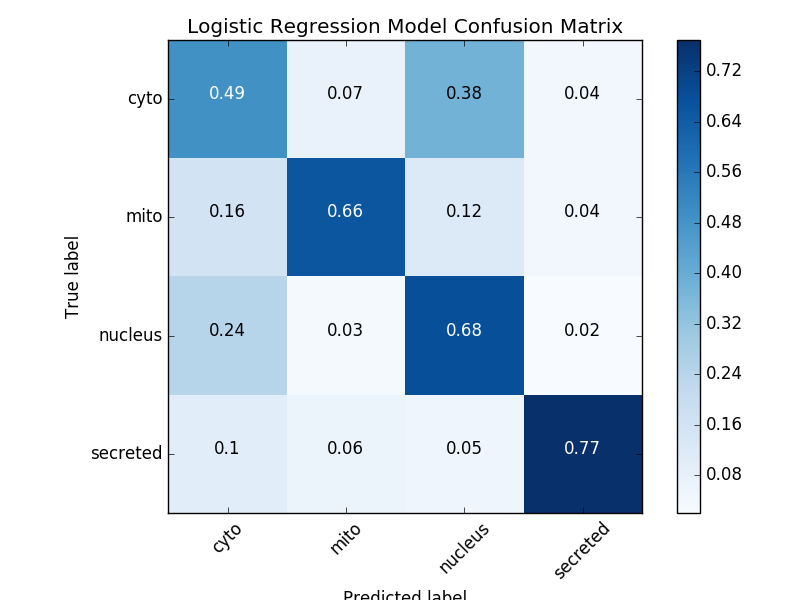
\includegraphics[width=235pt]{LR_cc.png}}
\caption{Logistic Regression Model}\label{fig:01}
\end{figure}

\begin{figure}[H]%figure1
\centerline{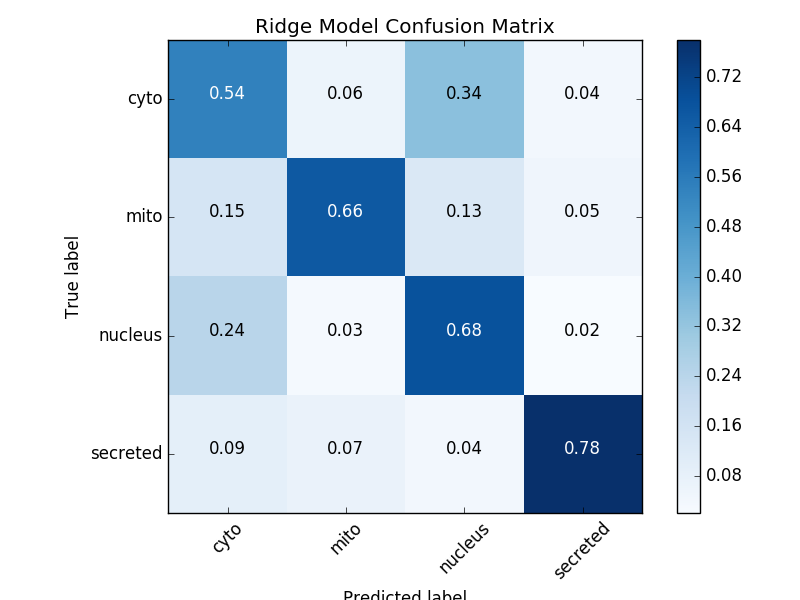
\includegraphics[width=235pt]{Ridge_cc.png}}
\caption{Ridge Regression Model}\label{fig:02}
\end{figure}

\begin{figure}[H]%figure1
\centerline{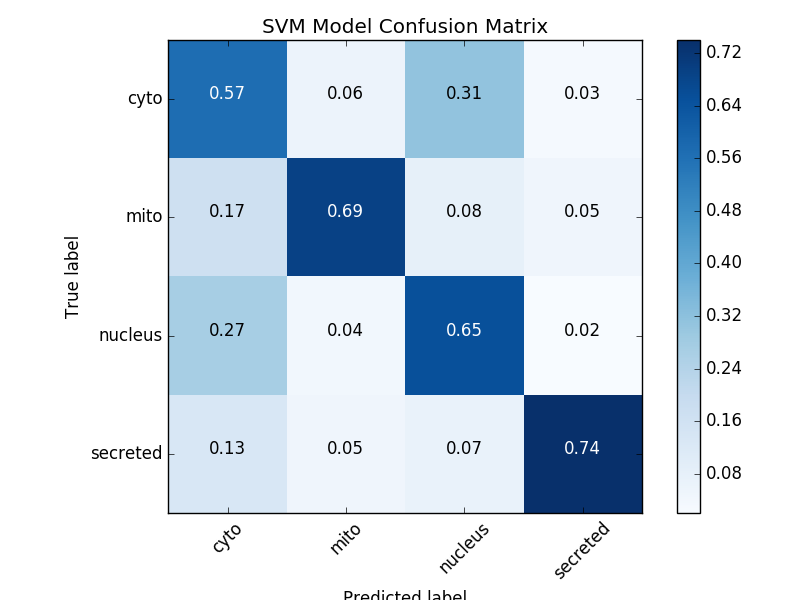
\includegraphics[width=235pt]{SVM_cc.png}}
\caption{SVM Model}\label{fig:03}
\end{figure}


\begin{figure}[H]%figure1
\centerline{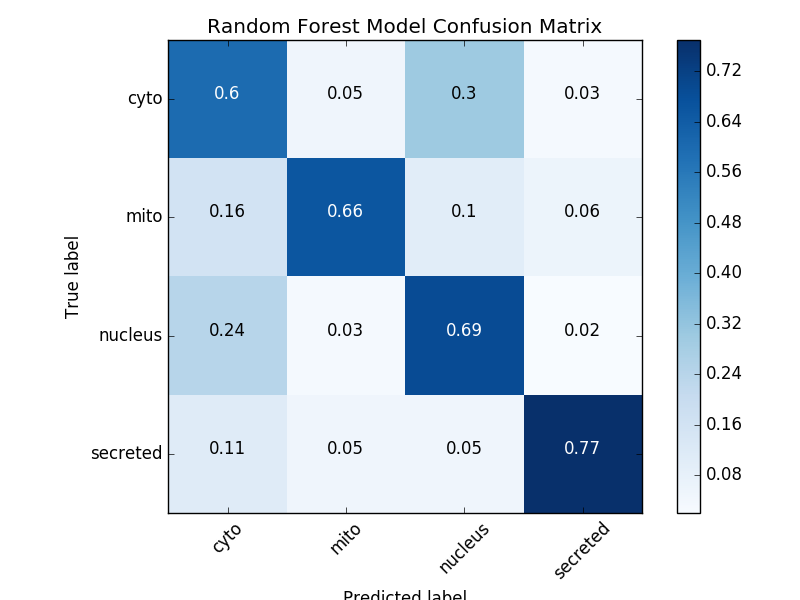
\includegraphics[width=235pt]{RF_cc.png}}
\caption{Random Forest Model}\label{fig:04}
\end{figure}


As it can be noticed, all the models have very similar confusion matrices. All of them seem to struggle identifying \textbf{cyto} class properly and mainly confuses it with the \textbf{nucleus} class. This also explains why the \textbf{ensemble model} doesn't seem to help. Indeed, if all the models have the same \textbf{weaknesses}, combining them will not improve the overall results. \\

This suggests that some supplementary features are needed in order to distinguish the \textbf{cyto} and \text{nucleus} class from each other. According, to what is presented in the research literature on the subject, these features are most likely going to be \textbf{sequence-related} such as the presence of a specific patern in the protein.

\subsection{Confidence on Mistakes}

\begin{table}[H]
\processtable{Confidence on erroneous prediction \label{Table:02}} {
\begin{tabular}{@{}llllll@{}}

\toprule 
True Label & cyto & mito & nucleus & secreted & \textbf{average}\\
\midrule
Random Forest Classifier &  0.527 & 0.453 & 0.498 & 0.442 & \textbf{0.497}\\
\botrule

\end{tabular}}{}
\end{table}

This idea is confirmed by the fact, on average, the model is not too confident when it is making a mistake as the confidence for these cases is around $50\%$. This confirms that, either a bigger training set size or adding some more features might help.  


\subsection{Prediction on blind test set}

As required by the Assignment, you can find bellow the subcellular localization predictions realized on a blind test.\\


\begin{minipage}{\linewidth}
SEQ677 Cyto Confidence 36\% \\
SEQ231 Cyto Confidence 30\% \\
SEQ871 Secreted Confidence 68\% \\
SEQ388 Nucleus Confidence 78\% \\
SEQ122 Nucleus Confidence 69\% \\
SEQ758 Nucleus Confidence 81\% \\
SEQ333 Cyto Confidence 47\% \\
SEQ937 Cyto Confidence 68\% \\
SEQ351 Cyto Confidence 52\% \\
SEQ202 Mito Confidence 71\% \\
SEQ608 Mito Confidence 78\% \\
SEQ402 Mito Confidence 67\% \\
SEQ433 Secreted Confidence 35\% \\
SEQ821 Secreted Confidence 79\% \\
SEQ322 Nucleus Confidence 90\% \\
SEQ982 Nucleus Confidence 82\% \\
SEQ951 Nucleus Confidence 46\% \\
SEQ173 Nucleus Confidence 57\% \\
SEQ862 Mito Confidence 66\% \\
SEQ224 Cyto Confidence 45\% \\
\end{minipage}
\end{methods}

\begin{thebibliography}{}

\bibitem[Saidi {\it et~al}., 2010]{Saidi2010}
R. Saidi, M. Maddouri and EM. Nguifo (2010) \\
Protein sequences classification by means of feature extraction with substitution matrices, {\it BMC Bioinformatics}

\bibitem[Q.-B. Gao {\it et~al}., 2005]{gao05}
Q-B Gao, Z-Z Wang, C Yan, Y-H Du (2005)\\ 
Prediction of protein subcellular location using a combined feature of sequence, {\it FEBS Letters}

\bibitem[Xua {\it et~al}., 2012]{Xua12}
D Xua, A Farmera, G Colletta, N V. Grishinb, Y M Chooka (2012)\\
Sequence and structural analyses of nuclear export signals in the NESdb database , {\it MBoC}

\end{thebibliography}

\newpage



\subsection{Main Code}
\twocolumn[{
\section{Appendix: Code}
\subsection{Main Code}
\lstinputlisting[language=Python, firstline = 1, lastline = 60]{main.py}
}]
\twocolumn[{
\lstinputlisting[language=Python, firstline = 61, lastline = 120]{main.py}
}]
\twocolumn[{
\lstinputlisting[language=Python, firstline = 121, lastline = 180]{main.py}
}]
\twocolumn[{
\lstinputlisting[language=Python, firstline = 181, lastline = 240]{main.py}
}]
\twocolumn[{
\lstinputlisting[language=Python, firstline = 241, lastline = 300]{main.py}
}]
\twocolumn[{
\lstinputlisting[language=Python, firstline = 301, lastline = 360]{main.py}
}]
\twocolumn[{
\lstinputlisting[language=Python, firstline = 361, lastline = 420]{main.py}
}]
\twocolumn[{
\lstinputlisting[language=Python, firstline = 421, lastline = 480]{main.py}
}]
\twocolumn[{
\lstinputlisting[language=Python, firstline = 481, lastline = 540]{main.py}
}]
\twocolumn[{
\lstinputlisting[language=Python, firstline = 540]{main.py}
}]
\twocolumn[{
\subsection{Tf-IDF Code}
\lstinputlisting[language=Python, firstline = 1, lastline = 60]{tf-idf.py}
}]
\twocolumn[{
\lstinputlisting[language=Python, firstline = 61, lastline = 120]{tf-idf.py}
}]
\twocolumn[{
\lstinputlisting[language=Python, firstline = 121]{tf-idf.py}
}]



\end{document}
